\documentclass[border=10pt]{standalone}
% Shared preamble for the VibeStack report diagrams.
% Build one diagram: pdflatex fig_x.tex && pdftoppm -r 220 -png -singlefile fig_x.pdf ../images/fig_x
\usepackage[T1]{fontenc}
\usepackage{lmodern}
\renewcommand{\familydefault}{\sfdefault}
\usepackage{tikz}
\usetikzlibrary{arrows.meta,positioning,shapes.geometric,shapes.misc,fit,backgrounds,calc}
\definecolor{vsred}{RGB}{204,0,0}
\definecolor{lay1}{RGB}{232,240,254}
\definecolor{lay2}{RGB}{230,246,236}
\definecolor{lay3}{RGB}{255,243,224}
\definecolor{lay4}{RGB}{243,232,253}
\tikzset{
  box/.style={draw, rounded corners=3pt, align=center, minimum height=0.95cm, inner sep=5pt, fill=white, font=\small},
  sbox/.style={box, minimum width=2.6cm},
  arrow/.style={-{Stealth[length=2.4mm]}, thick},
  darrow/.style={arrow, dashed},
  lbl/.style={font=\scriptsize, fill=white, inner sep=1.5pt},
  decision/.style={draw, diamond, aspect=2.1, align=center, inner sep=1pt, font=\small, fill=white},
  term/.style={draw, rounded rectangle, minimum width=2.4cm, minimum height=0.9cm, font=\small\bfseries, fill=white},
}

\usetikzlibrary{shapes.multipart}
\begin{document}
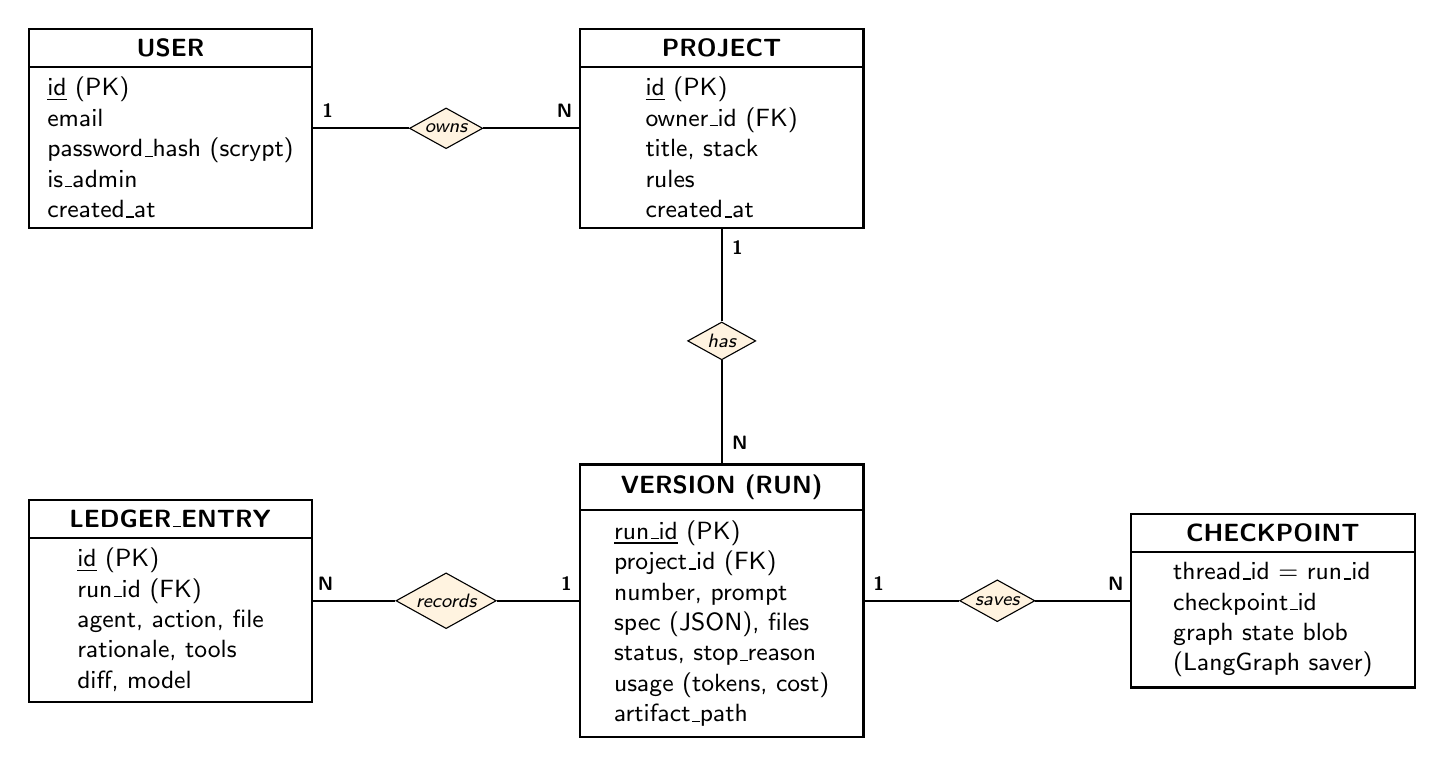
\begin{tikzpicture}
\tikzset{
  ent/.style={draw, thick, rectangle split, rectangle split parts=2, align=left, font=\small, fill=white, minimum width=3.6cm, rectangle split part fill={lay1,white}},
  rel/.style={draw, diamond, aspect=1.8, font=\scriptsize\itshape, fill=lay3, inner sep=1pt},
  card/.style={font=\scriptsize\bfseries}
}
\node[ent] (user) at (0,0) {\textbf{USER}\nodepart{two}\underline{id} (PK)\\email\\password\_hash (scrypt)\\is\_admin\\created\_at};
\node[ent] (proj) at (7,0) {\textbf{PROJECT}\nodepart{two}\underline{id} (PK)\\owner\_id (FK)\\title, stack\\rules\\created\_at};
\node[ent] (ver) at (7,-6) {\textbf{VERSION (RUN)}\nodepart{two}\underline{run\_id} (PK)\\project\_id (FK)\\number, prompt\\spec (JSON), files\\status, stop\_reason\\usage (tokens, cost)\\artifact\_path};
\node[ent] (led) at (0,-6) {\textbf{LEDGER\_ENTRY}\nodepart{two}\underline{id} (PK)\\run\_id (FK)\\agent, action, file\\rationale, tools\\diff, model};
\node[ent] (ck) at (14,-6) {\textbf{CHECKPOINT}\nodepart{two}thread\_id = run\_id\\checkpoint\_id\\graph state blob\\(LangGraph saver)};
\node[rel] (r1) at (3.5,0) {owns};
\node[rel] (r2) at (7,-2.7) {has};
\node[rel] (r3) at (3.5,-6) {records};
\node[rel] (r4) at (10.5,-6) {saves};
\draw[thick] (user) -- node[card, above, pos=0.15]{1} (r1) -- node[card, above, pos=0.85]{N} (proj);
\draw[thick] (proj) -- node[card, right, pos=0.2]{1} (r2) -- node[card, right, pos=0.8]{N} (ver);
\draw[thick] (ver) -- node[card, above, pos=0.15]{1} (r3) -- node[card, above, pos=0.85]{N} (led);
\draw[thick] (ver) -- node[card, above, pos=0.15]{1} (r4) -- node[card, above, pos=0.85]{N} (ck);
\end{tikzpicture}
\end{document}
